The main motivation which leads us to look for another approach to be used is that we want to:
\begin{enumerate}
    \itemsep0em
    \item Use a small amount of data
    \item Have \textit{mild} assumptions on the noise.
\end{enumerate}

\section{Main ingredients}
In order to formulate the \textbf{Set-Membership System Identification problem} we need some important ingredient:
\begin{itemize}
    \itemsep0em
    \item We start from a discrete time \textit{parametrized regression form} 
    \begin{equation*}
        y(k) = f(y(k-1),...,y(k-n), u(k), u(k-1), u(k-m), \theta_1, ..., \theta_{n+m+1}), \quad m \le n
    \end{equation*}
    \item A-priori assumptions on the \textbf{system} $\mathcal{S}$:
    \begin{itemize}
        \item $m,n$ are known; 
        \item The function $f\in\mathcal{F}$ (for the moment we choose the LTI class of dynamical systems).
    \end{itemize}
    \item A-priori assumptions on the \textbf{noise}:
    \begin{itemize}
        \item Noise structure (\textbf{OE, EIV}); 
        \item The input and output noise is part of some \textbf{bounded sets} $\mathcal{B}$ and in particular:
        {\large{
            \begin{align*}
                &\eta(k)\in\mathcal{B}_\eta, \quad
                \xi(k) \in \mathcal{B}_\xi
            \end{align*}
        }}
    \end{itemize}
    Tipically the sets $\mathcal{B}$ are defined by \textbf{polynomial constraints}, it is common that
    {\large{
        \begin{equation*}
            \mathcal{B}_\eta = \{
                \eta: \ \vert \eta(k) \vert \le \Delta_\eta
            \}, \quad
            \mathcal{B}_\xi = \{
                \xi : \ \vert \xi(k) \vert \le \Delta_\xi
            \}
        \end{equation*}
    }}
\end{itemize}

The \textbf{key element} of the Set-Membership identification method is the research of the \textbf{Feasible parameter set (FPS)} that we denote with $\mathcal{D}_\theta$. In a nutshell, it is the set of the parameter $\theta$ such that all the conditions exposed are fullfilled.

\section{Noise structures}

\subsection{Error-In-Variable set-up (EIV)}
\begin{figure}[h]
    \centering 
    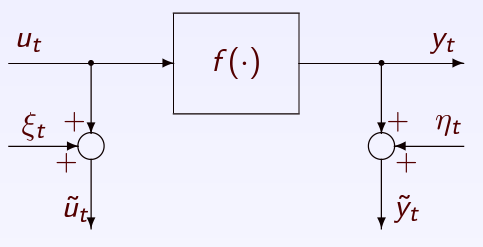
\includegraphics[scale=1]{images/EIV.png}
    \caption{EIV set-up}
\end{figure}
\textbf{Error-In-Variables (EIV)} problem refers to the most general case where the measurement noise is added both in the input and the output.\\
Due to the conditions we mentioned, we  have that:
{\large{
    \begin{equation*}
        \xi = [\xi(1) \quad ... \quad \xi(H)]\in \mathcal{B}_\xi, \quad
        \eta = [\eta(1) \quad ... \quad \eta(H)]\in \mathcal{B}_\eta
    \end{equation*}
}}

\subsection{Output-Error set-up(OE)}
\textbf{Output-Error(OE)} problem arises when the measurement noise $\eta$ enters only on the output of the system, while the system is assumed to be \textbf{exactly known}. [This is not strange to assume because sometimes one build the sequence of input to stimulate the system]. \\
Due to the condition we mentioned, we have that:
{\large{
    \begin{equation*}
        \eta = [\eta(1) \quad ... \quad \eta(H)]\in\mathcal{B}_\eta
    \end{equation*}
}}
\begin{figure}[h]
    \centering
    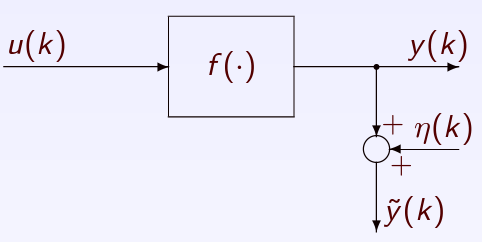
\includegraphics[scale=1]{images/OE.png}
    \caption{OE set-up}
\end{figure}

\section{Feasible Parameter Set (FPS)}
In the framework of \textbf{Set-Membership(SM) Identification}, all the parameters values consistent with the (i) \textit{a-priori information on the model}, (ii) \textit{a-priori information on the noise}, (iii) collected input/output data are considered as:
\begin{center}
    \large
    Feasible solution of the system identification problem
\end{center}
The set of all the parameters which satisfies these conditions is called the \textbf{Feasible Parameter Set}. For a \textbf{general EIV problem} it can be implicitly defined as:\\

\hspace*{-5mm}
\begin{tikzpicture}
\node [mybox] (box){%
    \begin{minipage}{.96\textwidth}    
        {\normalsize{
            \textbf{Feasible Parameter Set (FPS)}\\
    \begin{equation}
        \begin{aligned} \label{eq:FPS}
            \mathcal{D}_\theta = &\{
        \theta\in\mathbb{R}^p: \
        y(k)=f(y(k-1), ..., y(k-n), u(k),u(k-1), ..., u(k-m), \theta),\\
        & k=n+1,...,H,\\
        & y(k)=\tilde{y}(k)-\eta(k), \quad 
        u(k)=\tilde{u}(k)-\xi(k), \ k=1, ..., H\\
        &\vert \xi(k) \vert \le \Delta_\xi, \ 
        \vert \eta(k) \vert \le \Delta_\eta, \ 
        k=1,...,H
        \}
        \end{aligned}
    \end{equation}
}}
    \end{minipage}
};
\end{tikzpicture}%

\noindent
In the case that we want to identify a LTI discrete time system the set (\ref{eq:FPS}) is:
{\large{
    \begin{equation}
        \begin{aligned}
            \mathcal{D}_\theta =&\{
                \theta\in\mathbb{R}^p: \ 
                (\tilde{y}(k)-\eta(k))+
                \sum_{i=1}^n {\theta_i (\tilde{y}(k-1)-\eta(k-1))} =\\ &=\sum_{j=0}^m {\theta_j} (u(k-j)-\xi(k-j)), \ k=n+1, ..., H \\
                &\vert \xi(k) \vert \le \Delta_\xi, \ 
                \vert \eta(k) \vert \le \Delta_\eta, \ 
                k=1,...,H
            \}
        \end{aligned}
    \end{equation}    
}}

\noindent
The \textit{Feasible Parameter Set} enjoys the following properties:
\begin{enumerate}
    \itemsep0em
    \item The \textit{true value} of the parameter vector $\theta$ is guaranteed to belong to $\mathcal{D}_\theta$; 
    \item $\mathcal{D}_\theta$ implicitly quantify the uncertainty affecting the found mathematical model.
\end{enumerate}

Once we have found the FPS, we can use it to find \textbf{for each parameter} $\theta_k$ the \textit{Parameter Uncertainty Interval (PUI)} which is formally defined as
{\large{
    \begin{align}
            &PUI_k = [\underline{\theta}_k;\ \overline{\theta}_k], \\
        &\underline{\theta}_k=\min_{\theta\in\mathcal{D}_\theta} {\theta_k}, \quad \overline{\theta}=\max_{\theta\in\mathcal{D}_\theta} {\theta_k} \label{eq:PUIs}
    \end{align}
}}
The computation of $PUI_k$ requires to compute the \textbf{global optimal solution} of the optimization problems in (\ref{eq:PUIs}).

\subsection{Example \#1}
Let us suppose that the model to identify is a static system: a resistor.

\subsubsection{Ingredients}
\begin{enumerate}
    \item \textsc{A-priori information on the system}: $y(k)=\theta u(k)$
    \item \textsc{A-priori information on the noise} here we assume a \textbf{OE} noise structure, where $\vert \eta(k) \vert \le \Delta\eta$
    \item \textsc{A-posteriori info (I/O collected data)}, I have the pairs $[u(k), \tilde{y}(k)], k=1,...,H$
\end{enumerate}

\subsubsection{Feasible Parameter Set Computation}
{\large{
    \begin{align*}
        &\begin{aligned}
            \mathcal{D}_\theta = &\{
                \theta \in \mathbb{R}: y(k)=\theta u(k) \forall k=1,..., H \\
                &y(k)=\tilde{y}(k)-\eta(k), \quad \forall k=1,...,H\\
                &\vert \eta(k) \vert \le \Delta_\eta
            \}\Longleftrightarrow
        \end{aligned}\\ 
        &\begin{aligned}
            \mathcal{D}_\theta = &\{
                \theta \in \mathbb{R}: \tilde{y}(k)-\eta(k)=\theta u(k), \quad
                \vert \eta(k) \vert \le \Delta_\eta, \ 
                k=1,...,H 
            \}
        \end{aligned}\\
        &\begin{aligned}
            \mathcal{D}_\theta = &\{
                \theta \in \mathbb{R}: \eta(k)=\tilde{y}(k)-\theta u(k), \quad
                \vert \eta(k) \vert \le \Delta_\eta, \ 
                k=1,...,H 
            \}
        \end{aligned}\\
        &\begin{aligned}
            \mathcal{D}_\theta = \{
                \theta \in \mathbb{R}: \
                -\Delta_\eta \le \tilde{y}(k)-\theta u(k) \le \Delta_\eta, \quad
                k=1,...,H
            \}
        \end{aligned}\\
        &\begin{aligned}
            \mathcal{D}_\theta = \bigg\{
                \theta \in \mathbb{R}: \ 
                \theta \ge \frac{\tilde{y}(k)-\Delta_\eta}{u(k)}, \ \theta \le \frac{\tilde{y}(k)+\Delta_\eta}{u(k)}, \quad \forall k=1,...,H
            \bigg\}
        \end{aligned}
    \end{align*}
}}
In this case the FPS is the intersection between $H$ intervals, and the $PUI$ for the only parameter $\theta$ is coincident with this found interval.
We succeded in eliminating the dependence on $\xi,\eta$, but this was only  a particular case.\\
If only the system to identify had been only a little bit more complicated, the trick we used to eliminate $\eta$ from the set, would not have work. 

\section{Extended Feasible Parameter Set (EFPS)}
\noindent
This fact highlight the necessity to enlarge the FPS in such a way, it is able to contain also the variable $\theta, \xi$ which depends on the input and output error, defining the \textbf{Extended Feasible Parameter Set (EFPS)}.\\

\hspace*{-5mm}
\begin{tikzpicture}
\node [mybox] (box){%
    \begin{minipage}{.96\textwidth}     %Larghezza del box
        {\normalsize{
            \textbf{Extended feasible parameter set (EFPS)}\\
            \begin{equation}
                \begin{aligned}
                    \mathcal{D}_{\theta,\xi,\eta} =&\big\{
                        \theta\in\mathbb{R}^p,\ 
                        \xi \in \mathbb{R}^H, \
                        \eta \in \mathbb{R}^H: \ 
                        (\tilde{y}(k)-\eta(k))+ 
                        \sum_{i=1}^n {\theta_i (\tilde{y}(k-1)-\eta(k-1))} =\\ &=\sum_{j=0}^m {\theta_j} (u(k-j)-\xi(k-j)), \ k=n+1, ..., H \\
                        &\vert \xi(k) \vert \le \Delta_\xi, \ 
                        \vert \eta(k) \vert \le \Delta_\eta, \ 
                        k=1,...,H
                    \big\}
                \end{aligned}
            \end{equation} 
        }}
    \end{minipage}
};
\end{tikzpicture}%

This is the set of the parameters $\theta$ and noise samples $\xi, \eta$ which are consistent with the \textit{a-priori assumptions}. The FPS $\mathcal{D}_\theta$ we defined in the previous paragraphs is only the projection in the parameter space $\mathbb{R}^p$ of the EFPS $\mathcal{D}_{\theta,\xi,\eta}$.
Moreover the PUIs have to be computed on the extended space that in general is a \textbf{non-convex set} defined by \textbf{polynomial constraints}, in the following way:
{\large{
    \begin{equation}
        \underline{\theta}_k=\min_
        {\theta,\xi,\eta\in\mathcal{D_{\theta,\xi,\eta}}} {\theta_k}, \quad \overline{\theta}=\max_{\theta,\xi,\eta\in\mathcal{D_{\theta,\xi,\eta}}} {\theta_k} \label{eq:PUIs}
    \end{equation}
}}
One can wonder how to use the PUI for each parameter once you found it.  Usually for each $PUI_k$, the best choice is the \textbf{central estimate} $\theta_c$ defined as
\begin{equation*}
    \theta_{c,k} = \frac{\underline{\theta}_k+\overline{\theta}_k}{2}
\end{equation*}
By doing an example, there will be the possibility to better clarify some aspects even on the EFPS, that on the \textbf{central-estimate}, this gives us also the possibility to introduce some other theoretical aspects. 

\subsection{Example: First order system} 
Let us consider the problem of identifying a \textbf{first order system} of the form: 
\begin{equation*}
    y(k) = -\theta_1 y(k-1) + \theta_2 u(k)
\end{equation*}
The EFPS for such system is as following:
\begin{align*}
    \mathcal{D}_{\theta, \xi, \eta} = \big\{
        \theta \in \mathbb{R}^2, \xi \in \mathbb{R}^H, \eta \in \mathbb{R}^H: \ 
        &\tilde{y}(k)-\eta(k) = -\theta_1 \tilde{y}(k-1) + \theta_1 \eta(k-1) + \\
        &\theta_2 \tilde{u}(k) - \theta_2\xi(k) \forall k=2,..., H\\
        & \vert \eta(k) \vert \le \Delta_\eta, \ 
        \vert \xi(k) \vert \le \Delta_\xi
    \big\}
\end{align*}
We can note that the equations are exactly the same, with the difference that the FPS $\mathcal{D}_\theta$ is a \textbf{projection} of the EFPS onto the \textbf{parameter space}.
This set is characterized by: 
\begin{itemize}
    \itemsep0em
    \item nonlinear \textbf{equality constraints}, in particular they are bilinear and in general non-convex!
    \item \textbf{linear inequality constraints}
\end{itemize}
The projection of the EFPS on $\mathcal{D}_\theta$ is a non-convex set which can have some strange shape. The figure below constitutes an example of the FPS for the proposed Set-Membership identification problem. The extremities of each $PUI$ is depicted. In this way we have obtain the minimum (2D) hyper-rectangle which contains the Feasible Parameter Set.

\begin{figure}[h]
    \centering 
    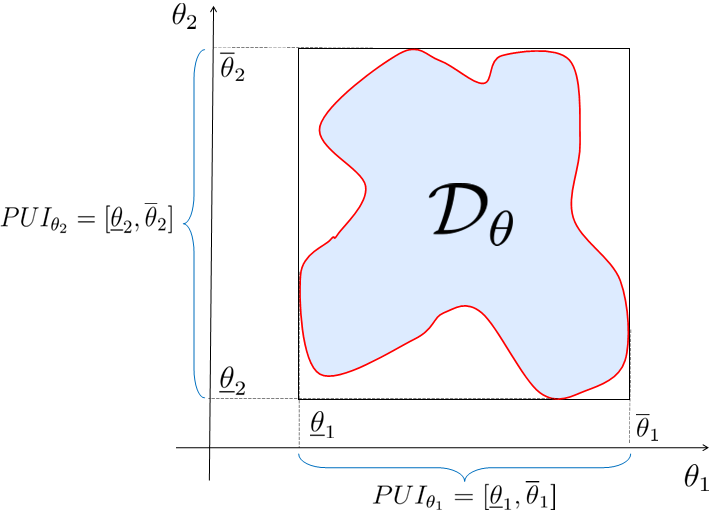
\includegraphics[scale=0.8]{FPS.png}
    \caption {FPS for a first order SysID problem}
\end{figure}
\noindent
After having completed the computation of the Parameter uncertainty intervals for all $\theta_k$, we can derive using the \textit{backward-shift operator} and the $\mathcal{Z}$-transform the \textbf{transfer function} of the agent
\begin{align*}
    G(z) &= \frac{\theta_2 z}{z+\theta_1}\\
    &  \text{where} \quad \theta_1 \in [\ \underline{\theta}_1, \ \overline{\theta}_1 \ ], \ \theta_2 \in [\ \underline{\theta}_2, \ \overline{\theta}_2 \ ]
\end{align*}
It is remarkable that for each point inside the set in blue we have a \textbf{different model}, but one can wonder: \textbf{How can we use this $PUI$?}
\begin{enumerate}
    \item If we are going to apply either robust control or robust simulation (for example using $\mathcal{H}_\infty, \mu$-synthesis and so on), this modelis already in the \textbf{correct form}!
    \item In other situations we would like to find a \textbf{single model} inside $\mathcal{D}_\theta$ to be used as the "best" (or \textbf{nominal model}). That is, we need to find a rule for selecting a single value of $(\theta_1, \theta_2)$ one single point inside the blue region. In this case it is a common choice to pick \textit{for each PUI} the \textbf{central estimate}
    {\large{
        \begin{equation*}
            \theta_k^c = \frac{\underline{\theta}_k+\overline{\theta}_k}{2}
        \end{equation*}
    }}
    \noindent
    this represents the center of the hyper-rectangle inside which the FPS lies. More rigorously, we define the \textbf{central estimate} as the solution of the following optimization problem:
    \begin{equation}
        \theta_c = \min_{\theta\in\mathbb{R}^2} \max_{\theta'\in\mathcal{D}_\theta} \Vert \theta-\theta' \Vert_\infty
    \end{equation}
    which is also known as the \textbf{Chebyshev center of $\mathcal{D}_\theta$ in $\ell_\infty$ norm}
\end{enumerate}
[Note that... in some particular cases the FPS might be so strange that is not connected, in this course the problems which arises these cases will not be discussed.]\\
This method is guaranteed to be a good choice inside the hyper-rectangle, however such center \textbf{is not guaranteed to be inside the FPS}. Consider for example the following case: 
\begin{figure}[h]
    \centering
    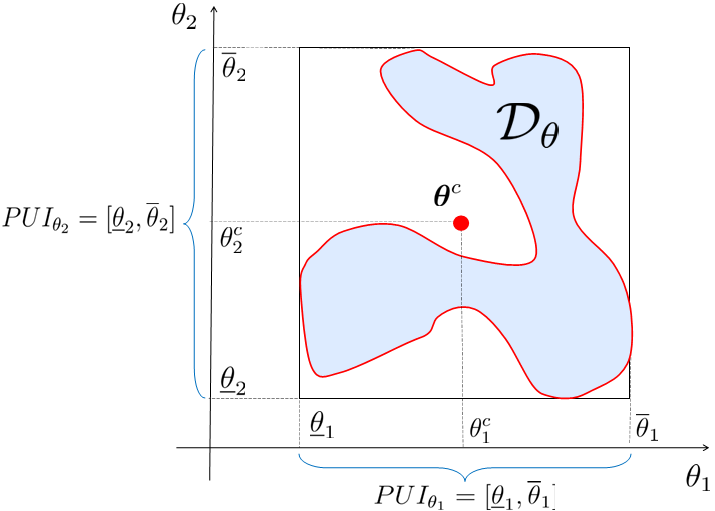
\includegraphics[scale=0.8]{FPS2.png}
    \caption{FPS with $\theta^c$ outside the set}
\end{figure}

\noindent
\textsf{[For this reason, it can be done another type of choice which is based on the use of the \textbf{conditional central estimate}, this and other related aspects are outside the purposes of this course].} 

\section{Convex relaxation for PUIs computation}
The fact that the feasible parameter set, in the most general caseof an EIV setting, is characterized by \textbf{bilinear constraints} can be used to note that \textbf{bilinearity} can be seen also as a special case of a \textbf{polynomial constraint}. We know that the FPS, as it is a projection of a non-convex set, itself it is not convex so we should solve a \textbf{non-convex optimization problem} which shows possibly a large number of local minima/maxima (optimal solution). Standard algorithm for nonlinear optimization are not able to compute the \textbf{global optimal solution}, that is the same to say that they potentially trap in local minima. \\
This is not a good news for us, since the intervals resulting from such local optimal solution cannot be qualified as PUIs, because it is not guaranteed that we can find $\theta_{\text{true}}$ inside them.\\

For the specific class of polynomial optimization problem (POP), powerful results are available to compute the solution which are based on the \textsf{Moment Theory} (Lassere). This tool can turn the original non-convex problem into a sequence of Semidefinite Programs (SDP) which instead are \textbf{convex}, their size depends on a parameter $\delta$ which is called the relaxation order.

The method is based on finding a convex approximation $\mathcal{D}^\delta_\theta$ for the FPS which is able to contain it. The higher the relaxation order $\delta$, the better the approximation. \\
It can be proved that when $\delta\to\infty$ a \textbf{convex hull} is obtained which is qualified as the smallest convex set which contains our (non-convex) FPS.

\begin{figure}[h]
    \centering
    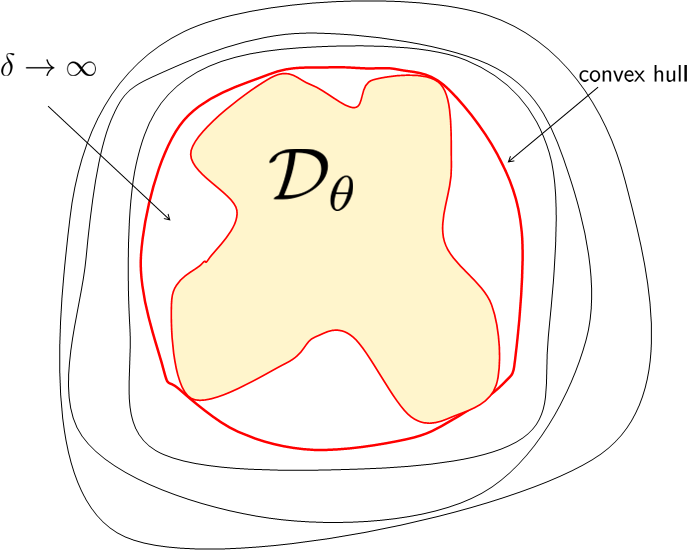
\includegraphics[scale=0.7]{relaxation.png}
\end{figure}


\noindent
The relaxation order has to have a minimum value which is:
\begin{equation}
        \delta_{min} = \max \bigg[
            \frac{deg(f_k(x))}{2}
    \bigg]
\end{equation}
where $f_k(x)$ are the constraints of the optimization problem. 
For any relaxation order $\delta$ which satisfies the constraint above, which is $\delta \ge \delta_{min}$ it is guaranteed that:
\begin{align*}
    \underline{\theta}_k^\delta \le \underline{\theta}_k, \quad 
    \overline{\theta}_k^\delta \ge \overline{\theta}_k \quad \forall k=1,...,n+m+1 
\end{align*}
Moreover it holds that:
{\Large{
    \begin{equation}
        \lim_{\delta\to\infty}  \underline{\theta}_k^\delta = \underline{\theta}_k, \quad
        \lim_{\delta\to\infty} \overline{\theta}_k^\delta = \overline{\theta}_k
    \end{equation}
}}
A \textbf{big disadvantage} of such relaxation method is the \textbf{computational complexity} that in particular grows exponentially in the relaxation order $\delta$. Therefore, the problem is tractable only in the case that $\delta$ is small. \\
The convex relaxation technique can be applied by using the freely available MATLAB tool \texttt{SparsePOP}. Given a POP, this tool automatically computes the convex SDP relaxation for a given relaxation order $\delta$. Finally, \texttt{SparsePOP} calls another software which is called \texttt{SeDuMi} in order to \textit{solve the SDP problems} obtained by convex relaxation.

\subsection{Solution of a generic POP using \texttt{SparsePOP}}
The tool \texttt{SparsePOP} is able to solve any optimization problem like:
{\large{
    \begin{align*}
        \min_{x\in\mathbb{R}^n}  \quad & f_0(x)\\
        &\text{s.t.}\\
        &f_k(x)\ge 0 \quad (k=1,...,l)\\
        &f_k(x)=0 \quad (k=l+1, ..., m)\\
        &\texttt{lb}_i \le x_i \le \texttt{ub}_i
    \end{align*}
}}
where $f_0,...,f_k$ are \textit{multivariate polynomial} function of the optimization variable $x\in\mathbb{R}^n$.
Let us introduce some examples in order to show how \texttt{SparsePOP} formulates the optimization problems, particular data structures has to be introduced for this aim.

\subsubsection{Example \#1 (general polynomial optimization problem)}
It is given the following optimization problem:
\begin{align*}
    \min_{x\in\mathbb{R}^3} \quad &(-2x_1+ 3x_2 -2 x_3) \\
    &\text{s.t.}\\
    &6x_1^2+3x_2^2-2x^2x_3 + 3x_3^2-17x_1+8x_2-14x_3 \ge -19\\
    &x_1 + 2 x_3 + x_3 \le 5\\
    &5x_2 + 3 x_3 \le 7\\
    &0\le x_1 \le 2, \quad 0 \le x_2 \le 2
\end{align*}
\noindent
\textsf{\large\textbf{SparsePOP formulation of the problem:}}\\
In the comments of the code we give some extra information, for further information see  the SparsePOP manual that is available online. \\
See: \href{URL} {https://sourceforge.net/projects/sparsepop/files/UserGuide.pdf/download}\\

\noindent
\textbf{\textsf{1) Objective function (data structures)}}

\begin{verbatim}
    objPoly.typeCone=1;         %always 1 here
    objPoly.dimVar=3;           %no opt. variables (including the constraints)
    objPoly.degree=1;           %degree of f_0
    objPoly.noTerms=3;          %number of monomials in f_0
    objPoly.supports=support;   %(matrix) see description below
    objPoly.coef=coef;          %(matrix) see description below         
\end{verbatim}
\texttt{support} and \texttt{coef} are data structures used to describe the objective function. In particular: 
\begin{itemize}
    \item \texttt{support} is a matrix with number of rows equal to \texttt{noTerms}, number of columns equal to \texttt{dimvar}, each entry of such matrix is a \textit{real number} which is the degree of the optimization variable involved in the \textbf{considered term}. In our case since we have ${f_0(x) = -2x_1+ 3x_2 -2 x_3}$ we have that \texttt{support} is equal to
    \begin{equation*}
        \texttt{support} = \begin{bmatrix}
            1&0&0\\
            0&1&0\\
            0&0&1
        \end{bmatrix}
    \end{equation*}
    it is only a case that it is an identity matrix.
    \item \texttt{coef} is a \textit{column vector} with coefficient of the different terms involved in $f_0(x)$. In our case we have that: 
    \begin{equation*}
        \texttt{coef} = \begin{bmatrix}
            -2\\3\\2
        \end{bmatrix}
    \end{equation*}
\end{itemize}

\noindent
\textbf{\textsf{2) Constraints (data structures)}}\\
The data structures related to the constraints are very similar, with the only difference that we need to put inequality constraints in the form $f_k(x)\ge0$. The following data structures have to be filled \textbf{for each constraint} of the optimization problem. Finally note that, in the code, the notation \texttt{ineqPolySys{1}} denotes the part of the data structure related to the first constraint.\\
Then, let us bring the first constraint of the optimization problem in a SparsePOP-compatible form:
\begin{equation*}
    f_1(x)=19-17x_1+8x_2-14x_3+6x_1^2+3x_2^2-2x_2x_3 +3x_3^2 \ge 0 
\end{equation*}
\begin{verbatim}
    ineqPolySys{1}.typeCone=1;        % 1 if >=, -1 if =
    ineqPolySys{1}.dimVar=3;          % the same as before
    ineqPolySys{1}.degree=2;          % inequality degree (deg max of the monomials)
    ineqPolySys{1}.noTerms=8;         % no terms in the inequality
    ineqPolySys{1}.support=support;   %as before
    ineqPolySys{1}.coef=coef;         %the same as before
\end{verbatim}

\noindent
Following the fashion of the previous step, let us define \texttt{support} and \texttt{coef}: 
\begin{equation*}
    \texttt{support} = \begin{bmatrix}
        0&0&0\\1&0&0\\
        0&1&0\\0&0&1\\
        2&0&0\\0&2&0\\
        0&1&1\\0&0&2
    \end{bmatrix}, \qquad 
    \texttt{coef} = \begin{bmatrix}
        19\\-17\\8\\-14\\
        6\\3\\-2\\3
    \end{bmatrix}
\end{equation*}

\noindent
\textbf{\textsf{3) Lower and upper bounds}}\\
The lower and upper bounds are indicated by employing two vectors called \texttt{lbd} and \texttt{ubd}, where respectively \texttt{lbd}=[\texttt{lb}$_i$,...,\texttt{lb}$_\textsf{dimVar}$], \texttt{ubd}=[\texttt{ub}$_i$,...,\texttt{ub}$_\textsf{dimVar}$]. In our example:
\begin{equation*}
    \texttt{ubd} = \begin{bmatrix}
        2\\1\\1e10
    \end{bmatrix}, \quad
    \texttt{lbd} = \begin{bmatrix}
        0\\0\\-1e10
    \end{bmatrix}
\end{equation*}
Where there are no upper and/or lower bound on a variable, mathematically speaking you should write $-\infty \le x_i \le +\infty$. Obviously in MATLAB we cannot use infinite values, for this reason we express this concept by introducing a very large number in the vector at the positions in which such bounds are required.

\subsubsection{Example \#2 (PUIs computation) ...\texttt{todo!()}}



 







